\section{Contribution of Supervised Losses to In-Between Instances Preservation} \label{sec:rq3}

The third research question addresses the role of supervision in enhancing the fidelity with which in-between instances (IBIs) are preserved in latent embeddings, specifically by examining how supervised losses perform in comparison to their unsupervised counterparts. The central focus lies on two well-established supervised objectives, the triplet margin loss and the cosine embedding loss, both of which explicitly incorporate label information to enforce relational constraints in the latent space. Unlike the unsupervised settings explored previously, where the model was restricted to structural cues emerging from reconstruction objectives or unsupervised preservation losses, the supervised setting benefits from additional knowledge of cluster and IBI labels. This enables the training process to anchor the embeddings more firmly in semantic distinctions, with the aim of improving cluster separability and transitional fidelity for IBIs.

To ensure comparability with earlier experiments and to isolate the effect of supervision, the autoencoder architecture and training configuration were kept constant throughout. For two-dimensional datasets, a 2–32–16–8–1 structure was employed, while three-dimensional datasets were modeled using a 3–64–32–16–2 architecture, both of which had been previously identified as optimal in the context of RQ-1 \ref{sec:rq1}. Training was consistently performed with the Adam optimizer, SELU activation functions, and a random sampling strategy, ensuring stable convergence and robust learning dynamics. Batch sizes were fixed at 16 for 2D data and 32 for 3D data, as these values had demonstrated superior performance and reliable convergence. By maintaining these parameters invariant, the study was able to attribute observed differences in IBI preservation directly to the effects of supervised loss functions rather than to confounding architectural or optimization factors.

% 2DBlobsS
\begin{figure}[htbp]
  \centering
  % subfigure 1
  \begin{subfigure}[b]{1.0\textwidth}
    \centering
    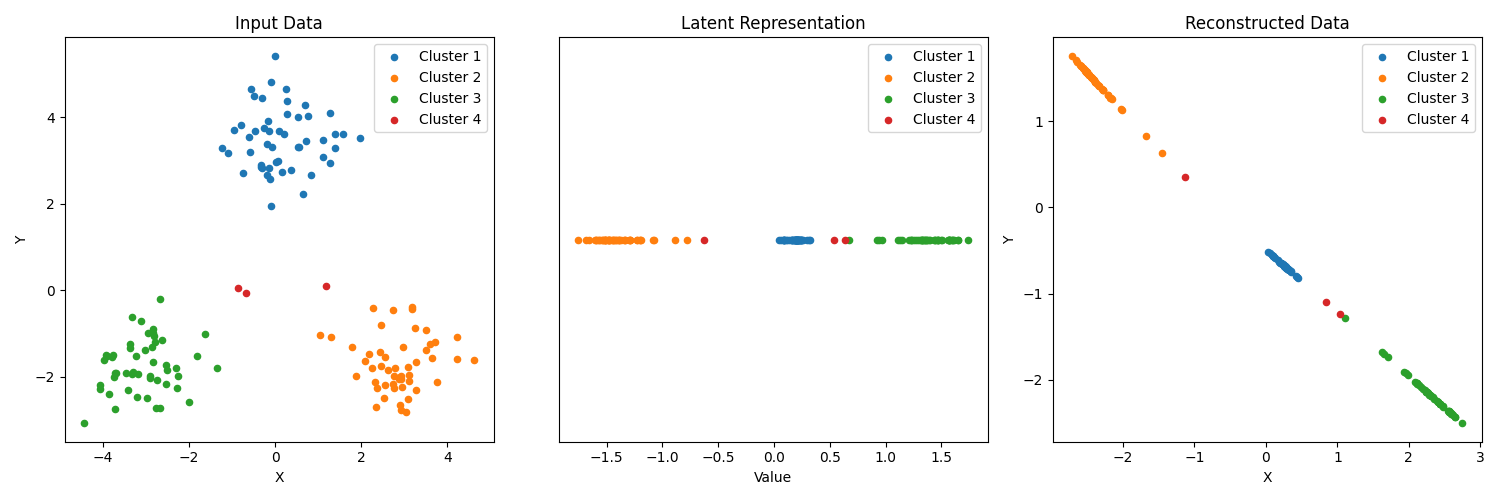
\includegraphics[width=\linewidth]{images/RQ3/tri/2DBlobsS_16_0.0001.png}
    \caption{n=16 with 0.0001 TriMarg.}
    \label{fig:RQ3/tri/2DBlobsS}
  \end{subfigure}
  \hfill
  % subfigure 2
  \begin{subfigure}[b]{1.0\textwidth}
    \centering
    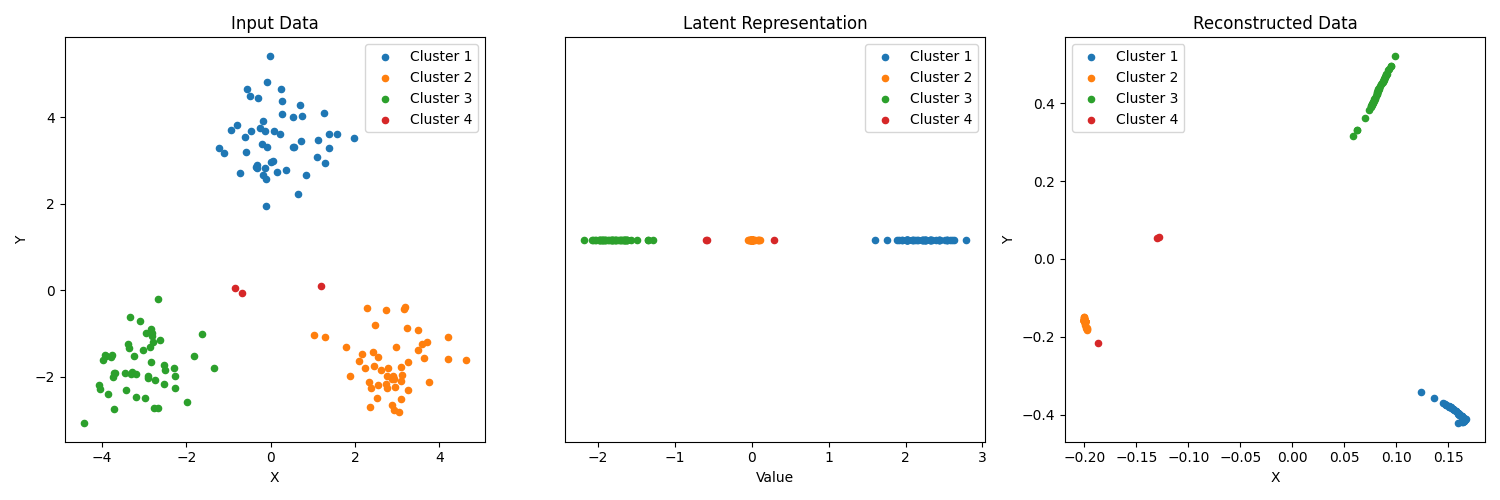
\includegraphics[width=\linewidth]{images/RQ3/cos/2DBlobsS_16_0.0001.png}
    \caption{n=16 with 0.0001 CosEmb.}
    \label{fig:RQ3/cos/2DBlobsS}
  \end{subfigure} 

  \caption{Comparison of 2DBlobsS dataset (153 instances) experiments with different
supervised loss functions.}
  \label{fig:RQ3/2DBlobsS}
\end{figure}

On the \textbf{2DBlobs} (Dataset \ref{fig:2DBlobsS}, Experiment \ref{fig:RQ3/2DBlobsS}) dataset, both supervised loss functions, the triplet margin loss and the cosine embedding loss, demonstrated strong performance in terms of cluster separation and IBI fidelity. In both cases, the clusters were distinctly separated with appropriate inter-cluster spacing that closely mirrored the structure of the original data, while the IBIs were positioned in faithful bridging locations that highlighted their transitional role. This reflects a clear advantage of introducing supervision, as the embeddings achieved both semantic separability and structural plausibility. Nonetheless, one notable limitation emerged consistently across both loss functions: the central cluster tended to collapse slightly, which disrupted the proportional balance among the clusters and led to a loss of relative size fidelity.

A further point of interest lies in the geometry of the reconstructed embeddings. Under cosine embedding loss, the reconstruction was organized on a two-dimensional manifold, preserving the overall dimensionality of the input space. In contrast, the triplet margin loss produced a representation that collapsed onto a near one-dimensional manifold. While this dimensional collapse might initially appear detrimental, it did not compromise the quality of the latent representation or the accurate placement of IBIs. Instead, it reflects a structural limitation of the autoencoder architecture itself rather than a failure of the loss function. In this sense, the reduced dimensionality highlights the way supervised constraints can dominate the embedding space, enforcing strong relational alignment even at the cost of manifold dimensionality, yet still preserving the essential fidelity of in-between instances.

% 2DBlobsM
\begin{figure}[htbp]
  \centering
  % subfigure 1
  \begin{subfigure}[b]{1.0\textwidth}
    \centering
    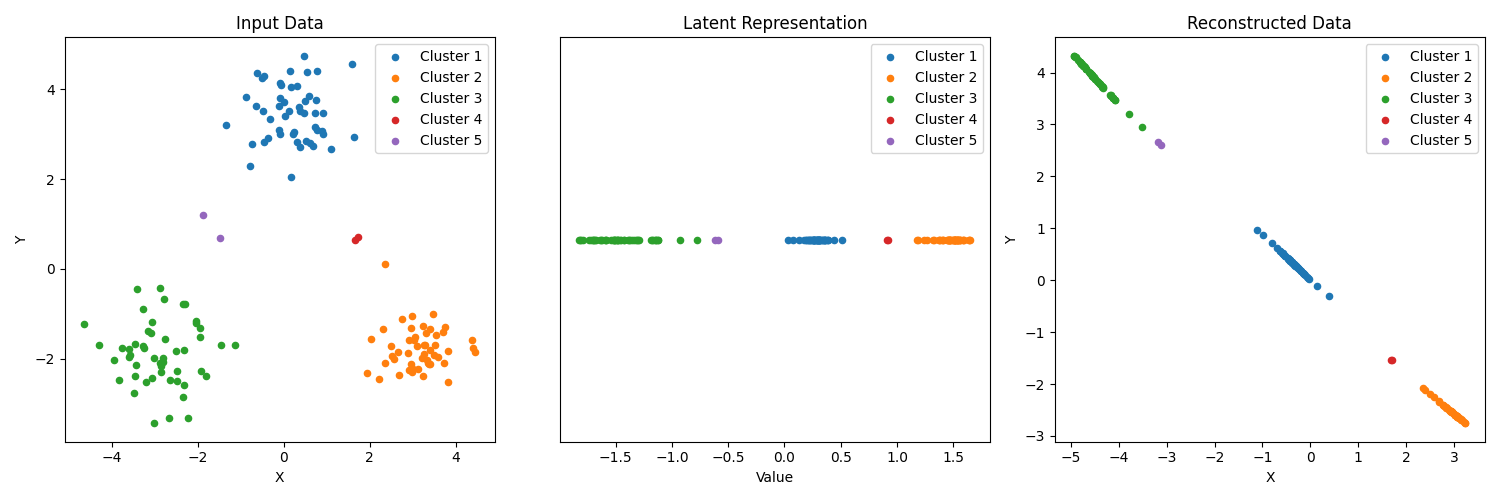
\includegraphics[width=\linewidth]{images/RQ3/tri/2DBlobsM_16_0.0001.png}
    \caption{n=16 with 0.0001 TriMarg.}
    \label{fig:RQ3/tri/2DBlobsM}
  \end{subfigure}
  \hfill
  % subfigure 2
  \begin{subfigure}[b]{1.0\textwidth}
    \centering
    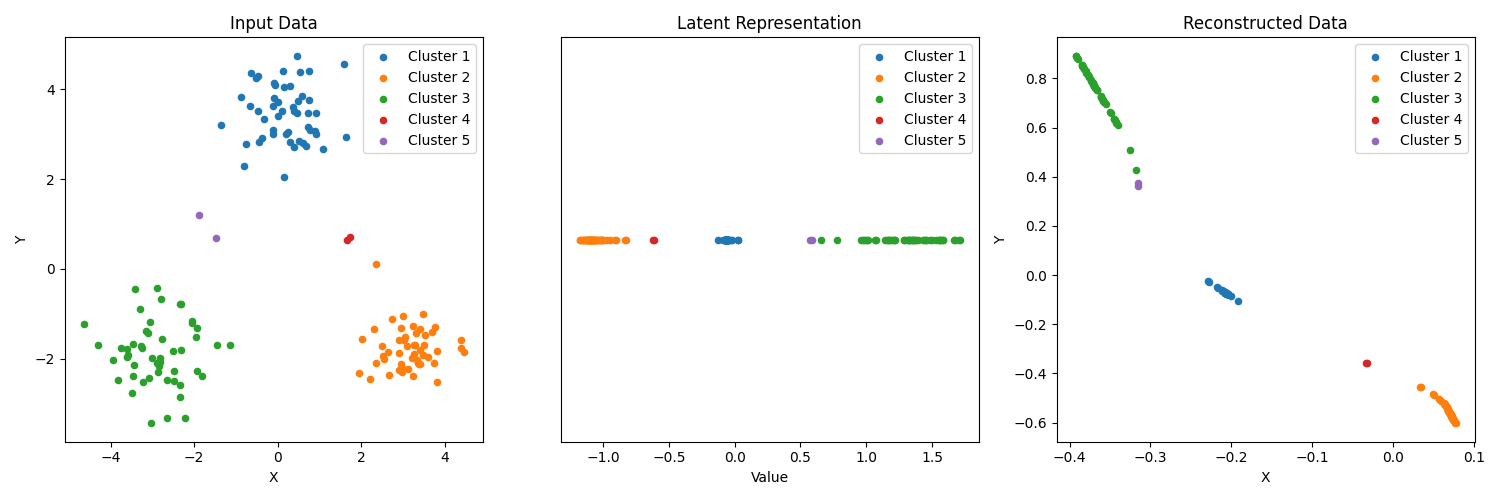
\includegraphics[width=\linewidth]{images/RQ3/cos/2DBlobsM_16_0.0011.png}
    \caption{n=16 with 0.0011 CosEmb.}
    \label{fig:RQ3/cos/2DBlobsM}
  \end{subfigure} 

  \caption{Comparison of 2DBlobsM dataset (154 instances) experiments with different
supervised loss functions.}
  \label{fig:RQ3/2DBlobsM}
\end{figure}

On the \textbf{2DBlobsM} (Dataset \ref{fig:2DBlobsM}, Experiment \ref{fig:RQ3/2DBlobsM}) dataset, the outcomes closely mirrored those observed for 2DBlobsS, which is unsurprising given the structural similarity between the two datasets. Both the triplet margin and cosine embedding losses once again produced well-separated clusters with IBIs placed convincingly in the transitional regions between them. The embeddings retained clear inter-cluster spacing and faithfully reflected the intended relationships among points. As with 2DBlobsS, however, the central clusters displayed a slight tendency to collapse, leading to a distortion of proportional cluster sizes. Yet this effect did not compromise the accurate positioning of IBIs or the overall separability of the latent space. In essence, the results on 2DBlobsM reaffirmed the consistency of the supervised approaches, showing that their advantages in IBI preservation generalize reliably across datasets with only minor structural variations.

% 2DMoons
\begin{figure}[htbp]
  \centering
  % subfigure 1
  \begin{subfigure}[b]{1.0\textwidth}
    \centering
    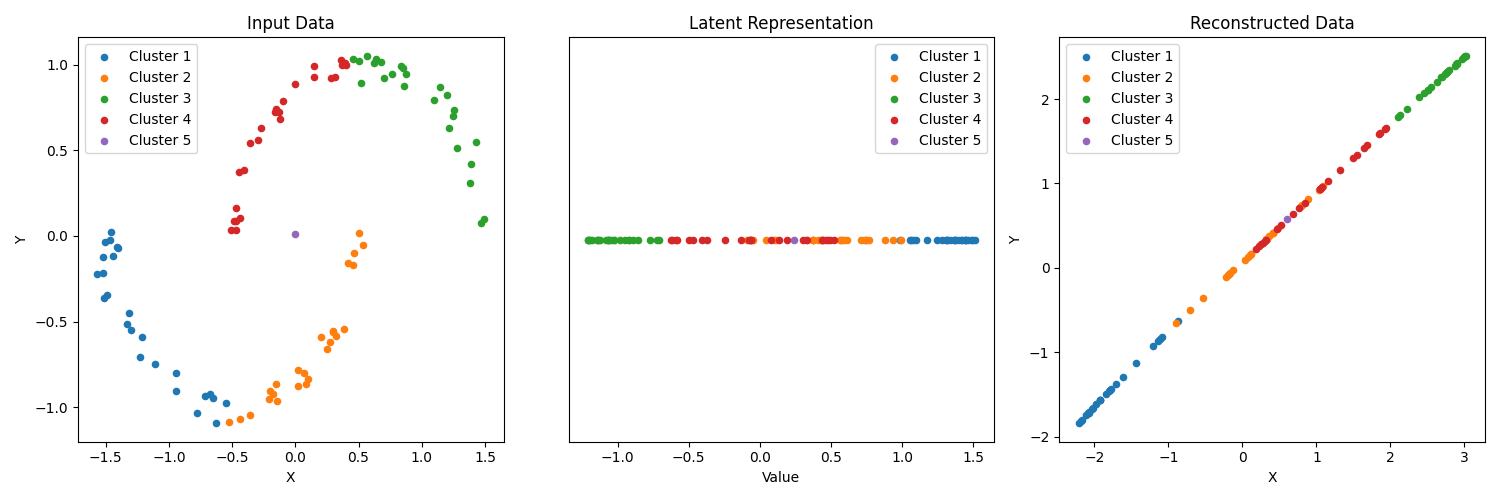
\includegraphics[width=\linewidth]{images/RQ3/tri/2DMoons_16_0.1762.png}
    \caption{n=16 with 0.1762 TriMarg.}
    \label{fig:RQ3/tri/2DMoons}
  \end{subfigure}
  \hfill
  % subfigure 2
  \begin{subfigure}[b]{1.0\textwidth}
    \centering
    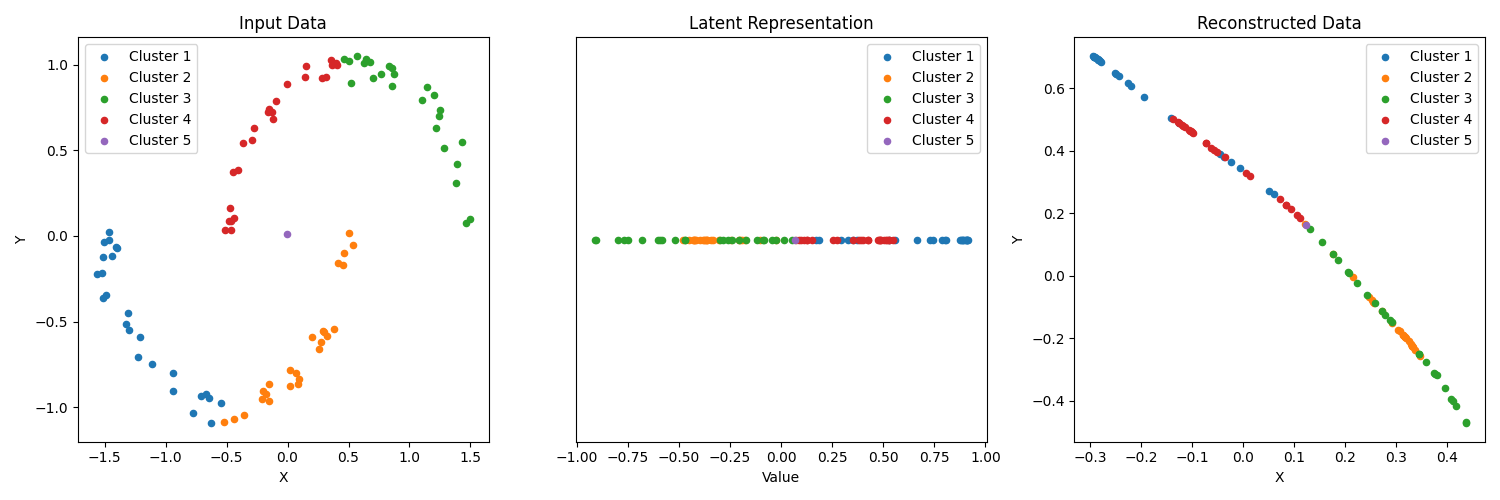
\includegraphics[width=\linewidth]{images/RQ3/cos/2DMoons_16_0.1309.png}
    \caption{n=16 with 0.1309 CosEmb.}
    \label{fig:RQ3/cos/2DMoons}
  \end{subfigure} 

  \caption{Comparison of 2DMoons dataset (101 instances) experiments with different
supervised loss functions.}
  \label{fig:RQ3/2DMoons}
\end{figure}

On the \textbf{2DMoons} (Dataset \ref{fig:2DMoons}, Experiment \ref{fig:RQ3/2DMoons}) dataset, both supervised configurations produced embeddings that collapsed into a near one-dimensional manifold. Given the nonlinear structure of the moons, this reduction in dimensionality may still be sufficient to capture the essential relationships of the dataset in a low-dimensional representation. Nevertheless, the two supervised losses differed notably in how they handled the delicate transitional region where the IBI is located. The triplet margin loss achieved a representation that preserved the overall shape of the moons reasonably well, but it struggled in the critical boundary zone: the IBI was not clearly distinguished, and the separation between the arcs became blurred at precisely the point where transitional fidelity was most important.

The cosine embedding loss, by contrast, performed even less effectively in this scenario. While it succeeded in separating the clusters, it embedded the sections of the moons in the wrong order, thereby distorting the dataset’s intrinsic geometry. This misalignment can be traced to the way the sections of each moon were treated as independent clusters during training. Such a setup conflicts with the dataset’s underlying structure, as the segments of a moon are not distinct clusters but rather parts of a continuous manifold. It is therefore reasonable to suspect that the poor performance under cosine embedding loss arises from this artificial cluster partitioning, and that treating each moon as a single coherent cluster would have allowed the loss function to preserve the structure more faithfully.

% 2DSwissRoll
\begin{figure}[htbp]
  \centering
  % subfigure 1
  \begin{subfigure}[b]{1.0\textwidth}
    \centering
    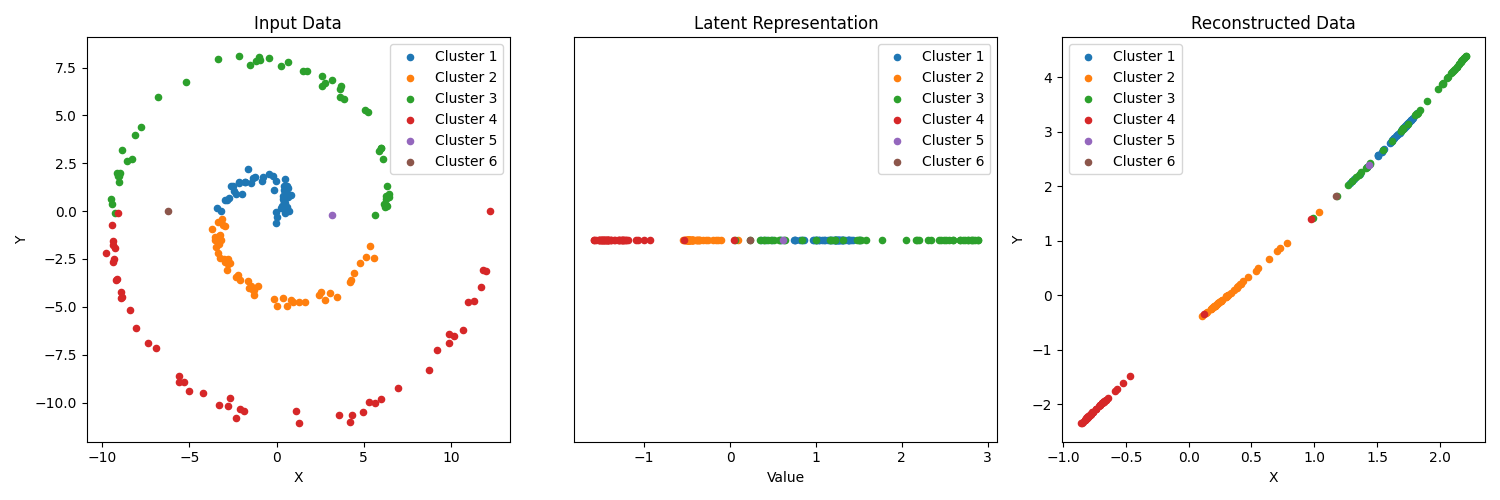
\includegraphics[width=\linewidth]{images/RQ3/tri/2DSwissRoll_16_0.0137.png}
    \caption{n=16 with 0.0137 TriMarg.}
    \label{fig:RQ3/tri/2DSwissRoll}
  \end{subfigure}
  \hfill
  % subfigure 2
  \begin{subfigure}[b]{1.0\textwidth}
    \centering
    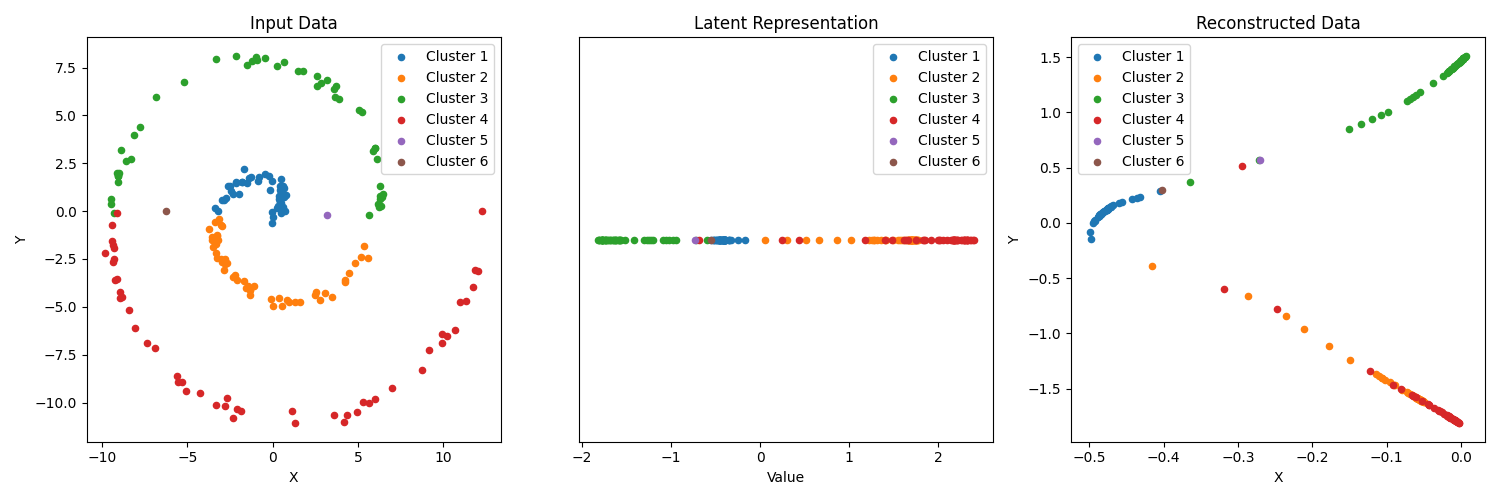
\includegraphics[width=\linewidth]{images/RQ3/cos/2DSwissRoll_16_0.0764.png}
    \caption{n=16 with 0.0764 CosEmb.}
    \label{fig:RQ3/cos/2DSwissRoll}
  \end{subfigure} 

  \caption{Comparison of 2DSwissRoll dataset (202 instances) experiments with different
supervised loss functions.}
  \label{fig:RQ3/2DSwissRoll}
\end{figure}

On the \textbf{2DSwissRoll} (Dataset \ref{fig:2DSwissRoll}, Experiment \ref{fig:RQ3/2DSwissRoll}) dataset, the same fundamental issue arose as in the 2DMoons experiment: the artificial treatment of contiguous sections of the manifold as separate clusters. This imposed structure led the supervised loss functions to enforce separability where continuity was in fact the defining property of the data. As a result, the different segments of the Swiss roll repelled each other in the latent space, breaking the sequential order that characterizes the manifold and thereby destroying its essential topology. Since this misrepresentation stems not from the loss functions themselves but from the experimental setup, further analysis of the results was not pursued, as the embeddings could not meaningfully reflect the intended structure of the dataset under these conditions.

% 3DBlobsS
\begin{figure}[htbp]
  \centering
  % subfigure 1
  \begin{subfigure}[b]{1.0\textwidth}
    \centering
    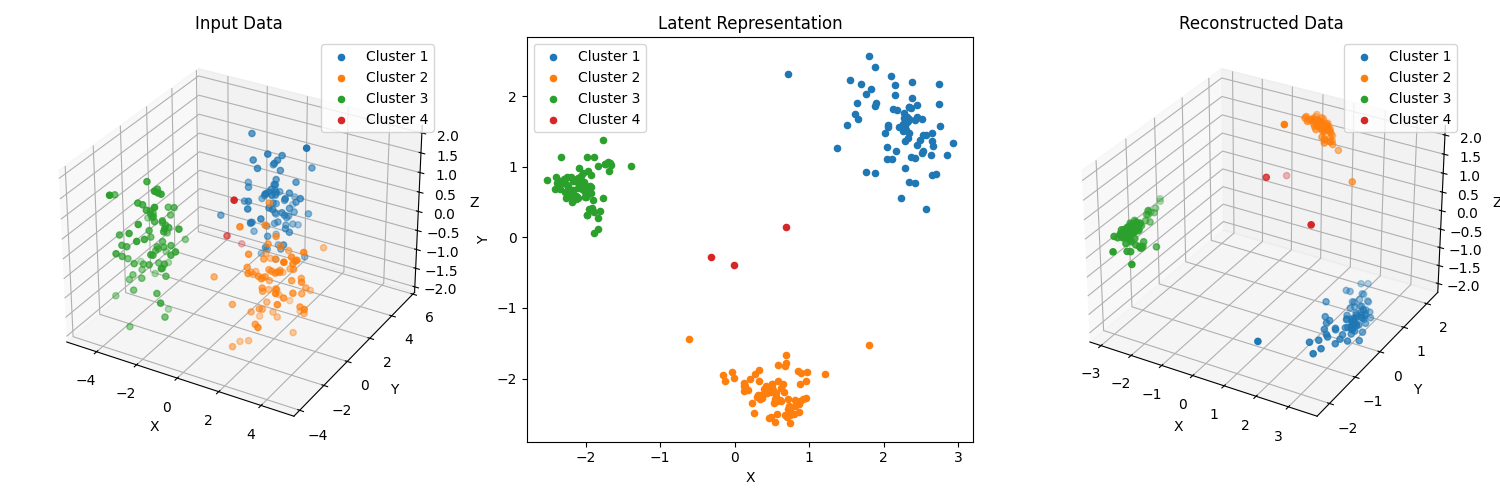
\includegraphics[width=\linewidth]{images/RQ3/tri/3DBlobsS_32_0.0001.png}
    \caption{n=32 with 0.0001 TriMarg.}
    \label{fig:RQ3/tri/3DBlobsS}
  \end{subfigure}
  \hfill
  % subfigure 2
  \begin{subfigure}[b]{1.0\textwidth}
    \centering
    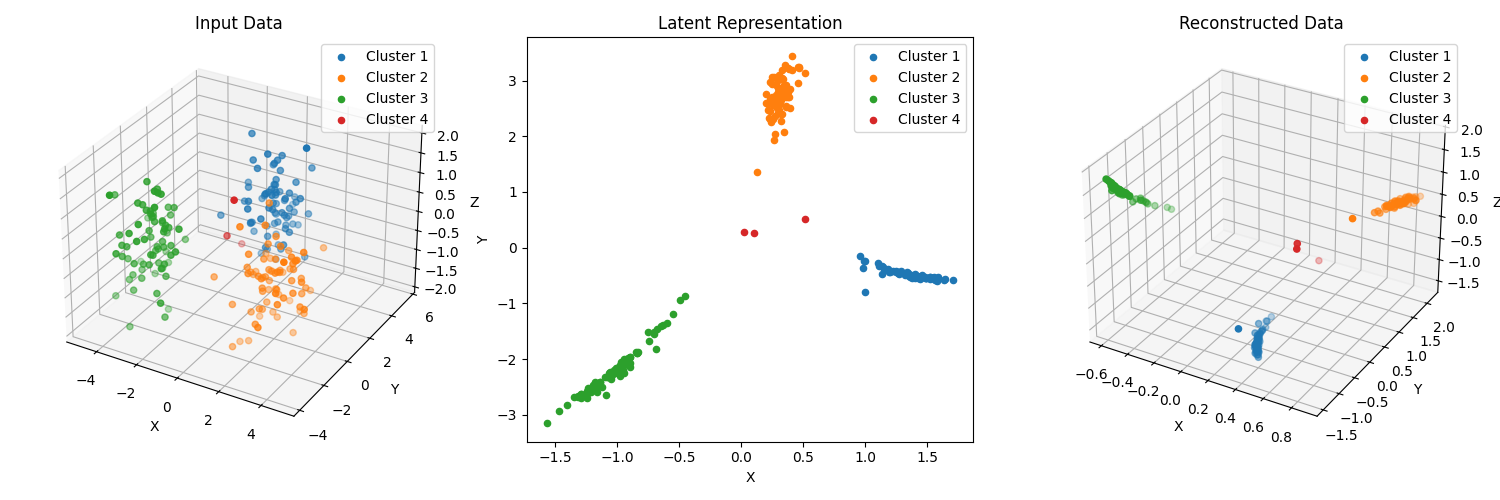
\includegraphics[width=\linewidth]{images/RQ3/cos/3DBlobsS_32_0.0001.png}
    \caption{n=32 with 0.0001 CosEmb.}
    \label{fig:RQ3/cos/3DBlobsS}
  \end{subfigure} 

  \caption{Comparison of 3DBlobsS dataset (228 instances) experiments with different
supervised loss functions.}
  \label{fig:RQ3/3DBlobsS}
\end{figure}

On the \textbf{3DBlobsS} (Dataset \ref{fig:3DBlobsS}, Experiment \ref{fig:RQ3/3DBlobsS}) dataset, both supervised loss functions succeeded in preserving the global structure of the data and, importantly, placed the IBIs convincingly in the center of the clusters, exactly where their transitional role would be expected. This demonstrates the strength of both triplet margin and cosine embedding losses in maintaining high-level relational fidelity between clusters and their in-between regions. However, when examining the finer details of the embeddings, clear differences emerged. Under cosine embedding loss, the local structure of the individual clusters was compromised: rather than maintaining compact, spherical formations, the clusters appeared elongated and distorted. This indicates that while cosine embedding was effective at enforcing global separability and IBI placement, it sacrificed some of the local geometry within clusters. Triplet margin loss, in contrast, preserved both the inter-cluster arrangement and the compactness of the clusters more faithfully, yielding an embedding that better reflected the original data distribution.

% 3DBlobsM
\begin{figure}[htbp]
  \centering
  % subfigure 1
  \begin{subfigure}[b]{1.0\textwidth}
    \centering
    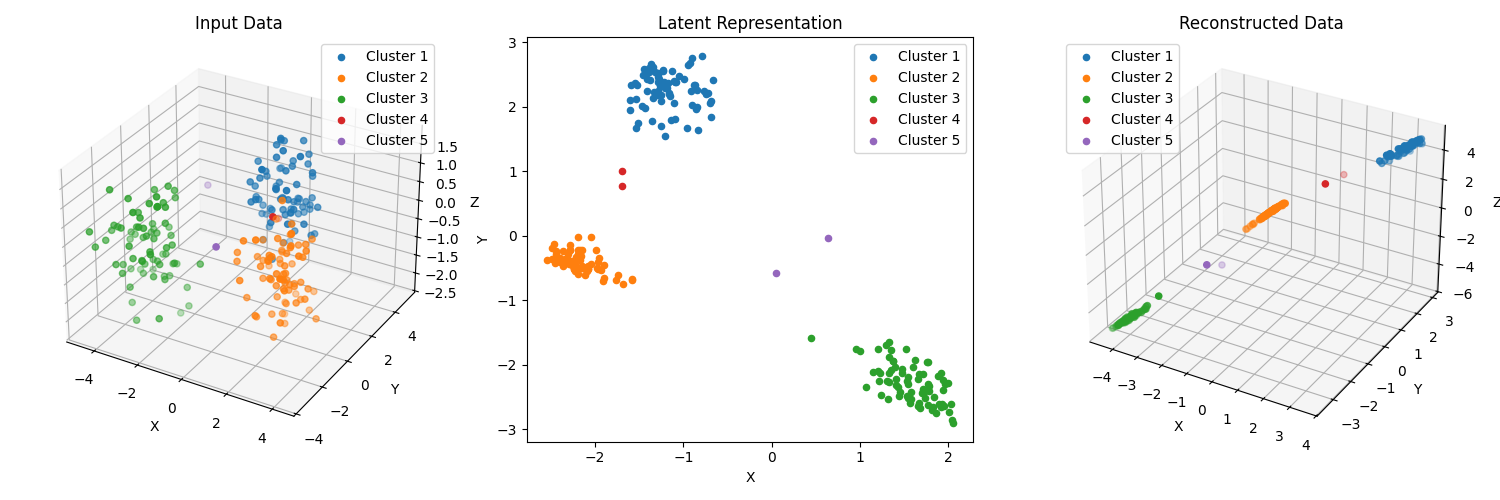
\includegraphics[width=\linewidth]{images/RQ3/tri/3DBlobsM_32_0.0001.png}
    \caption{n=32 with 0.0001 TriMarg.}
    \label{fig:RQ3/tri/3DBlobsM}
  \end{subfigure}
  \hfill
  % subfigure 2
  \begin{subfigure}[b]{1.0\textwidth}
    \centering
    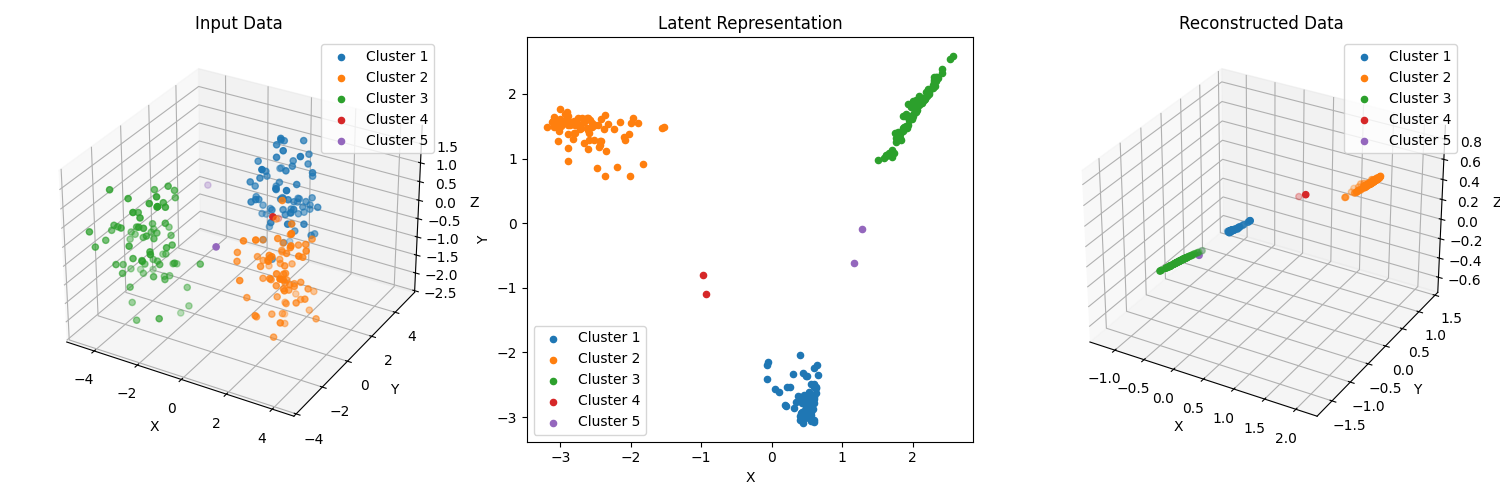
\includegraphics[width=\linewidth]{images/RQ3/cos/3DBlobsM_32_0.0019.png}
    \caption{n=32 with 0.0019 CosEmb.}
    \label{fig:RQ3/cos/3DBlobsM}
  \end{subfigure} 

  \caption{Comparison of 3DBlobsM dataset (229 instances) experiments with different
supervised loss functions.}
  \label{fig:RQ3/3DBlobsM}
\end{figure}

On the \textbf{3DBlobsM} (Dataset \ref{fig:3DBlobsM}, Experiment \ref{fig:RQ3/3DBlobsM}) dataset, the results closely resembled those obtained for 3DBlobsS, with both supervised approaches successfully preserving the overall separability of the clusters and positioning the IBIs in the expected transitional regions. Once again, cosine embedding loss produced elongated cluster representations, distorting the original spherical geometry and thereby failing to preserve the local structure of the clusters. Triplet margin loss avoided this elongation, but it introduced a different type of distortion at the global level: the relative distances between clusters were skewed. Specifically, the orange and blue clusters appeared closer to each other in the embedding space than they were to the green cluster, which does not correspond to the true spatial arrangement of the original data. Despite this discrepancy, the IBIs were still placed appropriately between the relevant clusters, indicating that both supervised losses retained the capacity to preserve transitional fidelity, even while compromising different aspects of the cluster structure.

% 3DMoons
\begin{figure}[htbp]
  \centering
  % subfigure 1
  \begin{subfigure}[b]{1.0\textwidth}
    \centering
    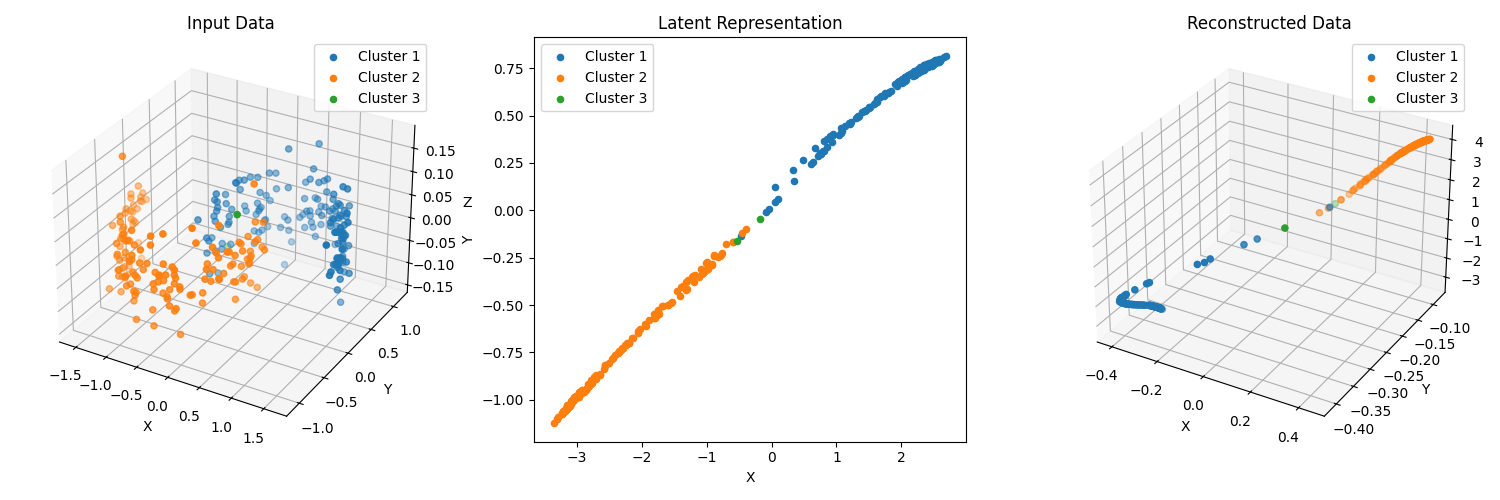
\includegraphics[width=\linewidth]{images/RQ3/tri/3DMoons_32_0.0001.png}
    \caption{n=32 with 0.0001 TriMarg.}
    \label{fig:RQ3/tri/3DMoons}
  \end{subfigure}
  \hfill
  % subfigure 2
  \begin{subfigure}[b]{1.0\textwidth}
    \centering
    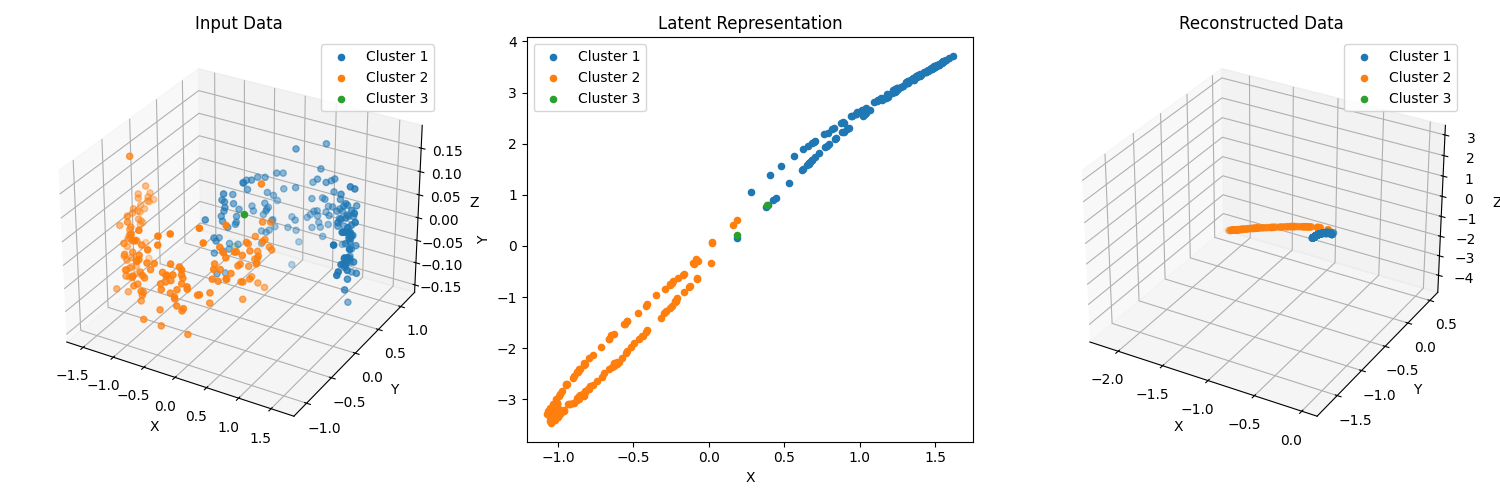
\includegraphics[width=\linewidth]{images/RQ3/cos/3DMoons_32_0.0069.png}
    \caption{n=32 with 0.0069 CosEmb.}
    \label{fig:RQ3/cos/3DMoons}
  \end{subfigure} 

  \caption{Comparison of 3DMoons dataset (302 instances) experiments with different
supervised loss functions.}
  \label{fig:RQ3/3DMoons}
\end{figure}

On the \textbf{3DMoons} (Dataset \ref{fig:3DMoons}, Experiment \ref{fig:RQ3/3DMoons}) dataset, it became evident that both supervised loss functions struggled to preserve the global structure of the clusters. The two moons collapsed into near one-dimensional manifolds, losing much of the curved three-dimensional geometry that characterizes the dataset. Despite this collapse, the embeddings still managed to place the IBIs convincingly in their transitional regions between the moons. This outcome suggests that, although the global cluster topology was not faithfully retained, the local neighborhood relationships were preserved sufficiently to maintain the relative positioning of IBIs. In other words, both triplet margin and cosine embedding losses were able to capture the local semantic structure required for IBI fidelity, even at the expense of accurately reconstructing the broader manifold shape.

% 3DSwissRoll
\begin{figure}[htbp]
  \centering
  % subfigure 1
  \begin{subfigure}[b]{1.0\textwidth}
    \centering
    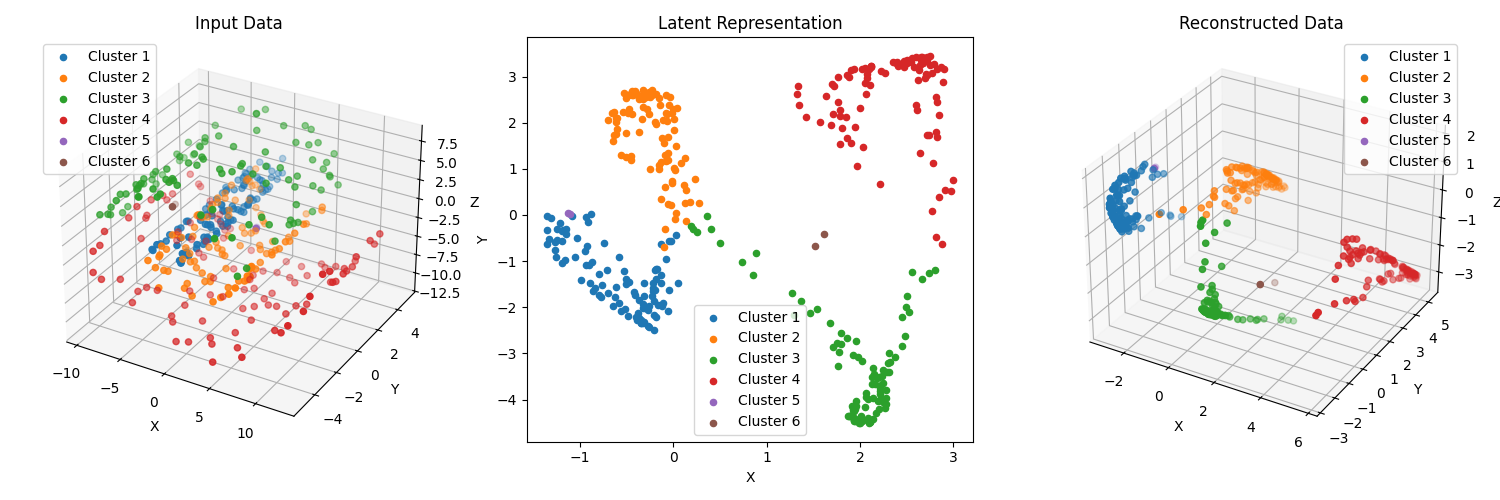
\includegraphics[width=\linewidth]{images/RQ3/tri/3DSwissRoll_32_0.0001.png}
    \caption{n=32 with 0.0001 TriMarg.}
    \label{fig:RQ3/tri/3DSwissRoll}
  \end{subfigure}
  \hfill
  % subfigure 2
  \begin{subfigure}[b]{1.0\textwidth}
    \centering
    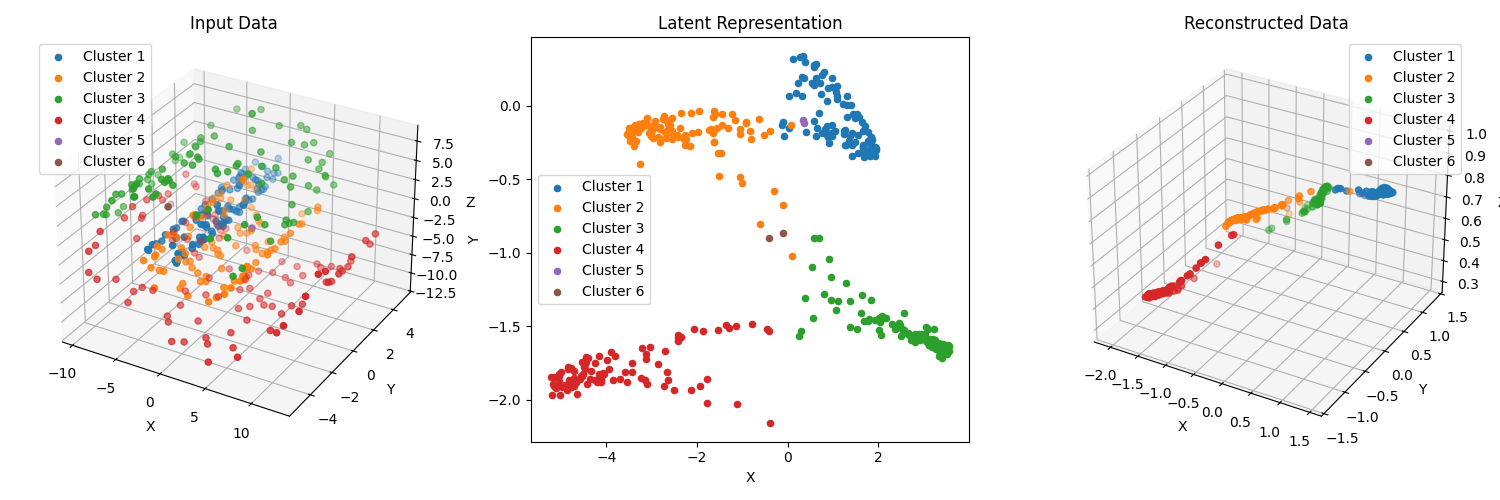
\includegraphics[width=\linewidth]{images/RQ3/cos/3DSwissRoll_32_0.0091.png}
    \caption{n=32 with 0.0091 CosEmb.}
    \label{fig:RQ3/cos/3DSwissRoll}
  \end{subfigure} 

  \caption{Comparison of 3DSwissRoll dataset (404 instances) experiments with different
supervised loss functions.}
  \label{fig:RQ3/3DSwissRoll}
\end{figure}

On the \textbf{3DSwissRoll} (Dataset \ref{fig:3DSwissRoll}, Experiment \ref{fig:RQ3/3DSwissRoll}) dataset, the supervised experiments produced results that were unexpectedly more favorable than those obtained in the two-dimensional case. Whereas the artificial labeling of contiguous sections had previously disrupted the embeddings by forcing separability where continuity was required, in three dimensions both loss functions succeeded in producing low-dimensional embeddings that unfolded the Swiss roll into a zigzag-like structure. This representation captured the global continuity of the manifold more convincingly, suggesting that the additional spatial degree of freedom allowed the supervised objectives to reconcile separation with manifold unfolding more effectively.

However, closer inspection revealed notable shortcomings, particularly in the treatment of IBIs. Under cosine embedding loss, the IBIs were absorbed into the body of the Swiss roll itself rather than occupying distinct bridging positions. This misplacement undermines the primary objective of IBI preservation, as the transitional role of these points was obscured. The triplet margin loss performed somewhat better in this regard, with the brown IBIs embedded in appropriate transitional zones between segments. Yet, even here, consistency was lacking, as other IBIs were not reliably preserved. This inconsistency suggests that while supervised losses can enhance the global unfolding of complex manifolds, they may not provide reliable mechanisms for consistently capturing the subtle transitional structures that IBIs represent.

% 3DTorus
\begin{figure}[htbp]
  \centering
  % subfigure 1
  \begin{subfigure}[b]{1.0\textwidth}
    \centering
    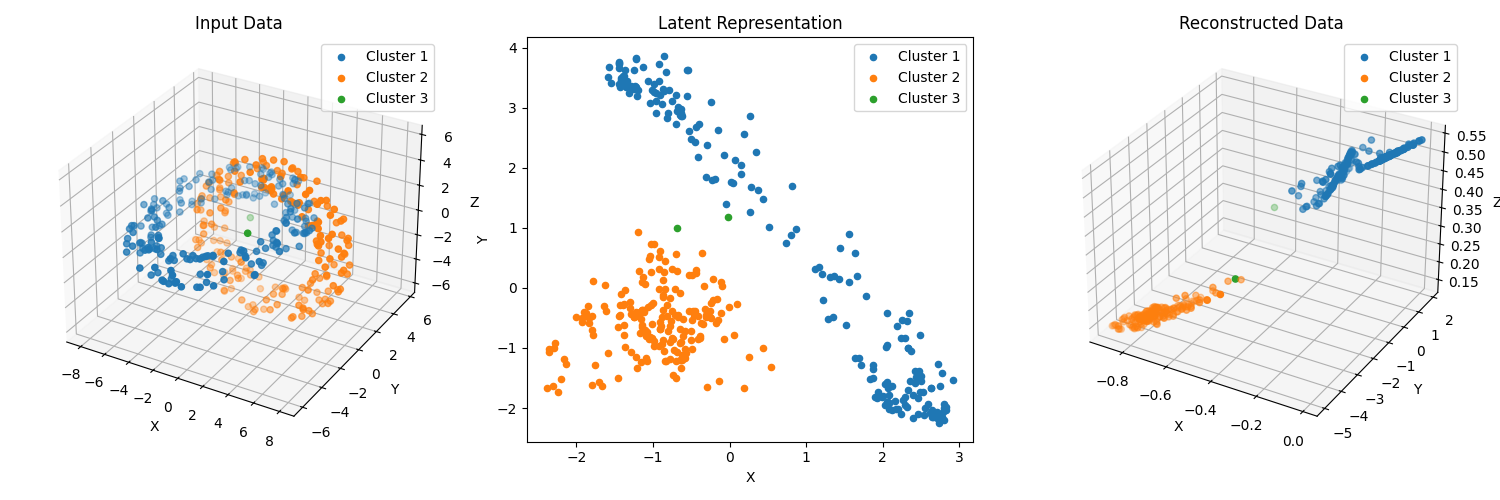
\includegraphics[width=\linewidth]{images/RQ3/tri/3DTorus_32_0.0190.png}
    \caption{n=32 with 0.0190 TriMarg.}
    \label{fig:RQ3/tri/3DTorus}
  \end{subfigure}
  \hfill
  % subfigure 2
  \begin{subfigure}[b]{1.0\textwidth}
    \centering
    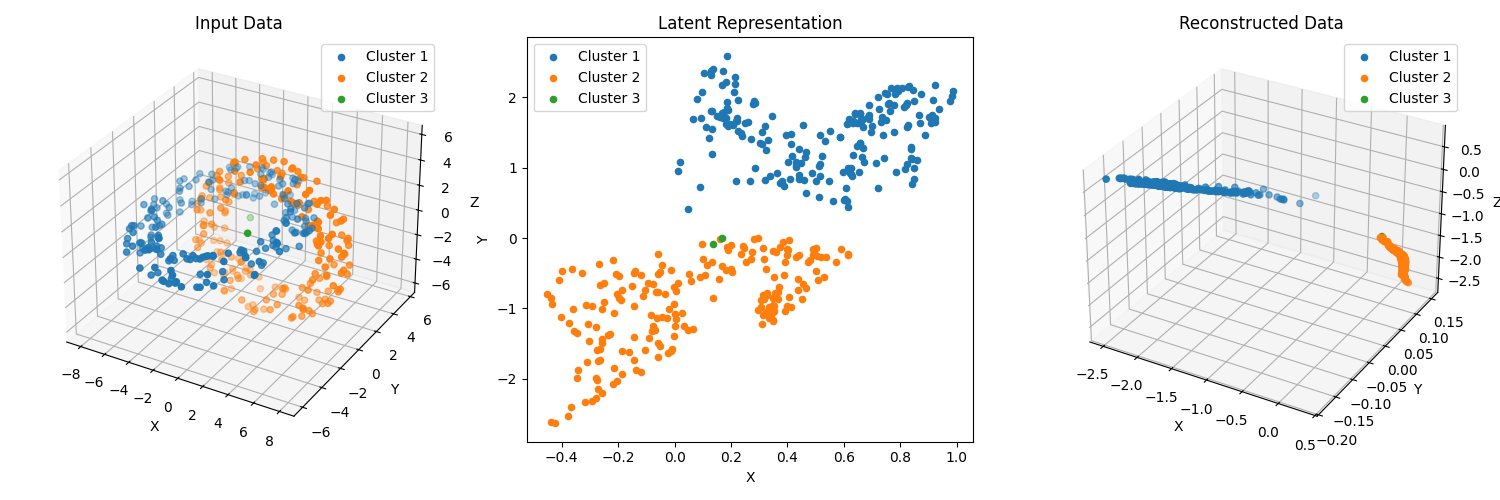
\includegraphics[width=\linewidth]{images/RQ3/cos/3DTorus_32_0.0013.png}
    \caption{n=32 with 0.0013 CosEmb.}
    \label{fig:RQ3/cos/3DTorus}
  \end{subfigure} 

  \caption{Comparison of 3DTorus dataset (402 instances) experiments with different
supervised loss functions.}
  \label{fig:RQ3/3DTorus}
\end{figure}

On the \textbf{3DTorus} (Dataset \ref{fig:3DTorus}, Experiment \ref{fig:RQ3/3DTorus}) dataset, the supervised losses yielded mixed and somewhat problematic results. The triplet margin loss successfully disentangled the two interwoven toroidal clusters and positioned the IBIs in between them, which at first glance reflects successful transitional fidelity. However, this came at the severe cost of global structure preservation: the toroidal topology was completely lost, with the clusters no longer resembling their original donut-shaped forms. In this sense, while the IBIs were correctly embedded, the broader geometric integrity of the dataset collapsed.

The cosine embedding loss, by contrast, retained the relative size proportions of the clusters more faithfully, avoiding the degree of distortion seen under triplet margin loss. Yet it failed in terms of IBI preservation: instead of occupying bridging positions, the IBIs collapsed onto the boundary of the orange cluster, losing their transitional identity. Moreover, as with the triplet margin configuration, the donut-like structure of the clusters themselves was not preserved, with the embedding failing to reflect the original toroidal geometry. Together, these outcomes highlight the difficulty both supervised objectives face when tasked with maintaining complex manifold structures: one objective succeeds in placing IBIs correctly but destroys cluster topology, while the other retains cluster proportions but loses the IBIs.

% 3DSphere
\begin{figure}[htbp]
  \centering
  % subfigure 1
  \begin{subfigure}[b]{1.0\textwidth}
    \centering
    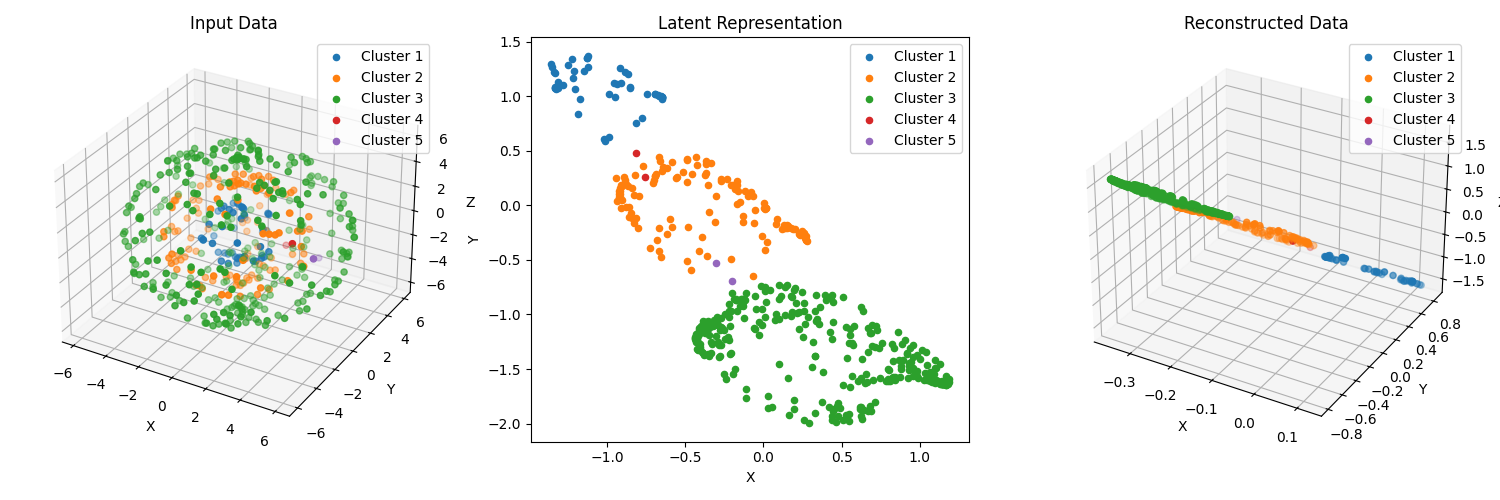
\includegraphics[width=\linewidth]{images/RQ3/tri/3DSphere_32_0.0001.png}
    \caption{n=32 with 0.0001 TriMarg.}
    \label{fig:RQ3/tri/3DSphere}
  \end{subfigure}
  \hfill
  % subfigure 2
  \begin{subfigure}[b]{1.0\textwidth}
    \centering
    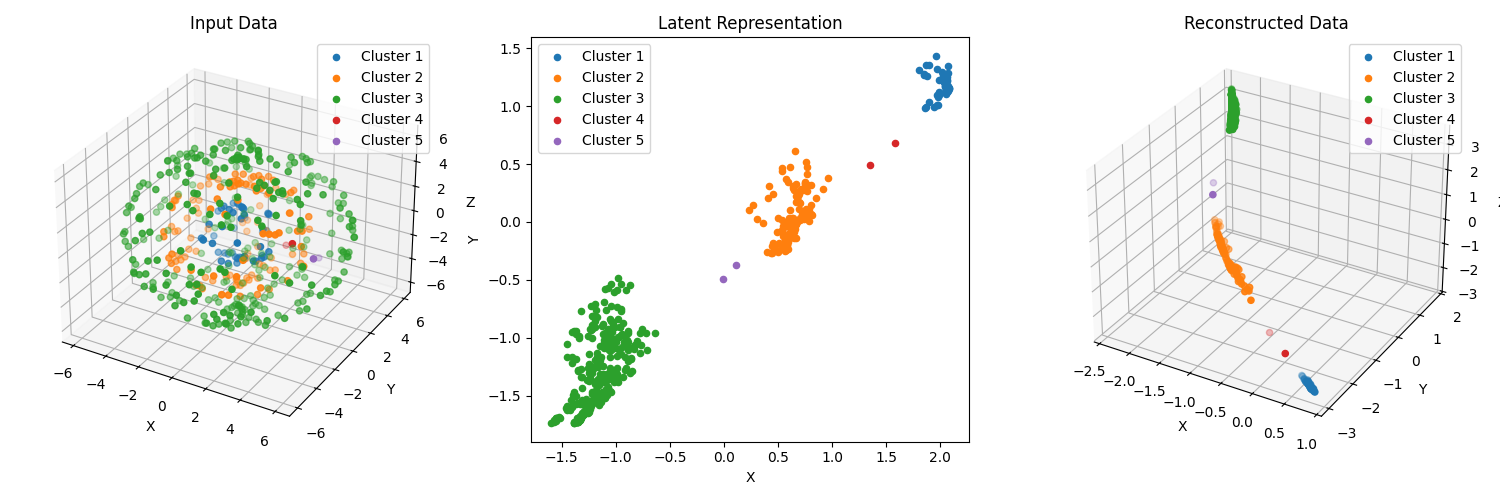
\includegraphics[width=\linewidth]{images/RQ3/cos/3DSphere_32_0.0017.png}
    \caption{n=32 with 0.0017 CosEmb.}
    \label{fig:RQ3/cos/3DSphere}
  \end{subfigure} 

  \caption{Comparison of 3DSphere dataset (492 instances) experiments with different
supervised loss functions.}
  \label{fig:RQ3/3DSphere}
\end{figure}

On the \textbf{3DSphere} (Dataset \ref{fig:3DSphere}, Experiment \ref{fig:RQ3/3DSphere}) dataset, the triplet margin loss delivered results that can be described as nearly ideal. The three spherical clusters were clearly separated, their relative size differences were preserved, and the IBIs were placed accurately in the bridging regions between the clusters. This outcome demonstrates the strength of the triplet margin objective in simultaneously maintaining global structure, local cluster fidelity, and transitional fidelity, making it one of the most successful configurations observed across all experiments.

Cosine embedding loss also achieved a respectable embedding in this setting: the clusters were well separated, and the IBIs were positioned in plausible transitional spaces. However, unlike the triplet margin loss, it failed to preserve the intrinsic spherical geometry of the clusters. Instead, the clusters appeared distorted, echoing the shortcomings already observed in earlier experiments where local shapes were sacrificed for global separability. This behavior closely paralleled the patterns seen with the soft trustworthiness loss in unsupervised configurations, reinforcing the impression that cosine embedding emphasizes relational separability at the expense of preserving manifold geometry.
\newline

The evaluation of the third research question reveals a consistent pattern across all datasets: in no case was the original dimensionality or structure of the data in the reconstruction fully preserved. Irrespective of the supervised loss employed, the embeddings collapsed into lower-dimensional manifolds, suggesting that a portion of the structural information was inevitably lost during the learning process. This dimensional reduction did not prevent the models from separating clusters and positioning IBIs in the latent space.

Across the experiments, both triplet margin and cosine embedding losses behaved in broadly similar ways, differing mainly in specific aspects of how cluster structures and IBIs were represented. A recurring observation was that both losses tended to sacrifice global cluster geometry, spherical, toroidal, or otherwise complex forms were rarely retained. However, they consistently succeeded in maintaining local relational information: clusters were separated in a semantically meaningful manner, and IBIs were, in most cases, embedded in appropriate transitional positions. This ability to preserve local fidelity, even at the cost of global structure, underscores the strengths and limitations of supervised loss objectives.

The most challenging datasets proved to be the 2D and 3D Moons, where both loss functions struggled to capture the curved manifold structures. In these cases, the embeddings collapsed too aggressively, and while IBIs were not entirely misplaced, the broader relational context was poorly represented. By contrast, in more complex datasets such as the 3DTorus or 3DSphere, both methods demonstrated a capacity to disentangle interwoven or encapsulated clusters, often achieving separability that most unsupervised objectives could not. Here, the triplet margin loss, in particular, distinguished itself, producing embeddings that better preserved inter-cluster relationships and more consistently positioned IBIs in their bridging roles. Overall, triplet margin loss outperformed cosine embedding loss in a greater number of scenarios, especially in cases where transitional fidelity and cluster separability needed to be simultaneously maintained.

Taken together, these findings suggest that while supervised losses represent a significant step forward in improving IBI preservation compared to purely unsupervised approaches, they are not without shortcomings. Both methods tend to be inconsistent in preserving global cluster geometry and local neighborhood simultaneously. The consistent dimensional collapse in reconstruction across all experiments indicates that valuable structural information is being discarded in the process. This points toward the need for hybrid strategies in future work. A promising direction would be to combine objectives such as triplet margin or cosine embedding with reconstruction-based losses like mean squared error. Such a combined objective could reconcile the strengths of both approaches: preserving the global manifold structure through reconstruction fidelity while simultaneously enforcing class-aware separability and transitional accuracy through supervised constraints.
